\documentclass[letterpaper]{sae}
\usepackage[spanish]{babel}%Para el español
\usepackage[utf8]{inputenc}%para los acentos
\PaperTitle{Implementación de una ALU en verilog sobre FPGA Spartan3E}
\AddAuthor{Morales Esteban, Salamandri Santiago, Uboldi Marino}{FCEFyN, UNC, Argentina}
\PaperNumber{Trabajo Páctico Nro. 1}
%\SAECopyright{1999}
\usepackage{graphicx} % Required for including pictures
\usepackage{float} % Allows putting an [H] in \begin{figure} to specify the exact location of the figure

\graphicspath{{Imagenes/}}

\usepackage{listings}

\usepackage{pxfonts}

\usepackage{color}
\usepackage{textcomp}
\definecolor{lbcolor}{rgb}{0.9,0.9,0.9}
\definecolor{gris_claro}{gray}{0.3}
\lstset{
	backgroundcolor=\color{lbcolor},
	tabsize=4,
	%rulecolor=,
	language=verilog,
        basicstyle=\scriptsize,
        upquote=true,
        aboveskip={1.5\baselineskip},
        columns=fixed,
        showstringspaces=false,
        extendedchars=true,
        breaklines=true,
        prebreak = \raisebox{0ex}[0ex][0ex]{\ensuremath{\hookleftarrow}},
        %frame=single,
        showtabs=false,
        showspaces=false,
        showstringspaces=false,
        identifierstyle=\ttfamily,
        keywordstyle=\bfseries \ttfamily ,%\color[rgb]{0,0,1}
        commentstyle=\itshape \ttfamily \color{gris_claro},%\color[rgb]{0.133,0.445,0.133}
        stringstyle=\ttfamily ,%\color[rgb]{0.627,0.126,0.941}
        numbers=left,                    % where to put the line-numbers; possible values are (none, left, right)
		numbersep=5pt,                   % how far the line-numbers are from the code
		numberstyle=\tiny,
}

\begin{document}
\maketitle
\section{abstract}
En computación, la unidad aritmético lógica, también conocida como ALU (siglas en inglés de arithmetic logic unit), es un circuito digital que calcula operaciones aritméticas (como suma, resta, multiplicación, etc.) y operaciones lógicas (si, y, o, no), entre dos números.

\section{Consigna Implementada}
\begin{itemize}
	\item Implementar una ALU sobre FPGA.
	\item Utilizar las placas de desarrollo Basys II.
	\item La ALU debe ser parametrizable (bus de datos) para poder ser utilizada posteriormente en el trabajo final.
	\item Validar el desarrollo por medio de Test Bench.
	\item La ALU deberá realizar las siguientes operaciones:
	\begin{center}
	\begin{tabular}{|c|c|}
		\hline 
		Operación & Código\tabularnewline
		\hline 
		\hline 
		ADD & 100000\tabularnewline
		\hline 
		SUB & 100010\tabularnewline
		\hline 
		AND & 100100\tabularnewline
		\hline 
		OR & 100101\tabularnewline
		\hline 
		XOR & 100110\tabularnewline
		\hline 
		SRA & 000011\tabularnewline
		\hline 
		SRL & 000010\tabularnewline
		\hline 
		NOR & 100111\tabularnewline
		\hline 
	\end{tabular}
	\end{center}
\end{itemize}

\section{Desarrollo}
Se implementa una ALU de 8 bits (bus de datos parametrizable) en FPGA, la cual se divide en 3 módulos:

\begin{itemize}
	\item Calculadora: Módulo encargado de instanciar los otros módulos.
	\item Cargador: Módulo encargado de inicializar los valores de los registros.
	\item ALU: Módulo encargado de realizar las operaciones tabuladas en los requerimientos.
\end{itemize}

\section{Descripción}
\subsection{Cargador}
\begin{verbatim}
cargador(entrada,boton_a,boton_b,
		boton_op,a,b,op);
\end{verbatim}

\begin{figure}[H] % Example image
\center{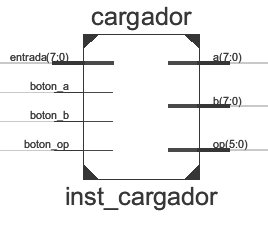
\includegraphics[width=0.7\linewidth]{cargador}}
\label{fig:cargador}
\end{figure}

\subsubsection{Entradas}
\begin{itemize}
	\item entrada: Es el registro de entrada de ancho de bus parametrizable.
	\item boton\_a: Cuando esta entrada está en '1' carga el valor de la entrada en la salida a;
	\item boton\_b: Cuando esta entrada está en '1' carga el valor de la entrada en la salida b;
	\item boton\_op: Cuando esta entrada está en '1' carga el valor de la entrada en la salida op;
\end{itemize}
\subsubsection{Salidas}
\begin{itemize}
	\item a: Este registro de salida será un operando de la ALU.
	\item b: Este registro de salida será un operando de la ALU.
	\item op: Este registro de salida será el código de operación de la ALU. 
\end{itemize}
\subsection{ALU}
\begin{verbatim}
alu(a,b,op,rdo,carry,zero);
\end{verbatim} 

\begin{figure}[H] % Example image
\center{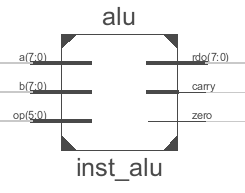
\includegraphics[width=0.7\linewidth]{alu}}
\label{fig:alu}
\end{figure}

\subsubsection{Entradas}
\begin{itemize}
	\item a: Este registro de entrada es un operando de la ALU.
	\item b: Este registro de entrada es un operando de la ALU.
	\item op: Este registro de entrada es el código de operación de la ALU.
\end{itemize}
\subsubsection{Variables Internas}
\begin{itemize}
	\item \begin{verbatim}
		wire [`BUS_DAT_MSB+1:0] resultado;
	\end{verbatim}
	Se utiliza una sola variable interna de tipo "wire" para almacenar el
	resultado de la función "funcion\_alu" 
\end{itemize}
\subsubsection{Salidas}
\begin{itemize}
	\item rdo: Este registro almacena el resultado de la operación de la ALU.
	\item carry: Este registro de un bit representa el carry de la operación.
	\item zero: Este registro de un bit es la bandera de zero de la operación.
\end{itemize}
\subsection{Calculadora}
\begin{verbatim}
module calculadora(entrada,boton_a,boton_b,
boton_op,rdo,carry,zero);
\end{verbatim}

\begin{figure}[H] % Example image
\center{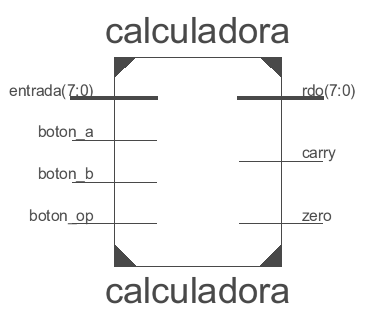
\includegraphics[width=0.7\linewidth]{calculadora}}
\label{fig:calculadora}
\end{figure}

Como la calculadora es el módulo que instancia a los otros dos módulos las entradas serán iguales a las entradas de uno
y las salidas serán iguales a las salidas del otro.

\begin{figure}[H] % Example image
\center{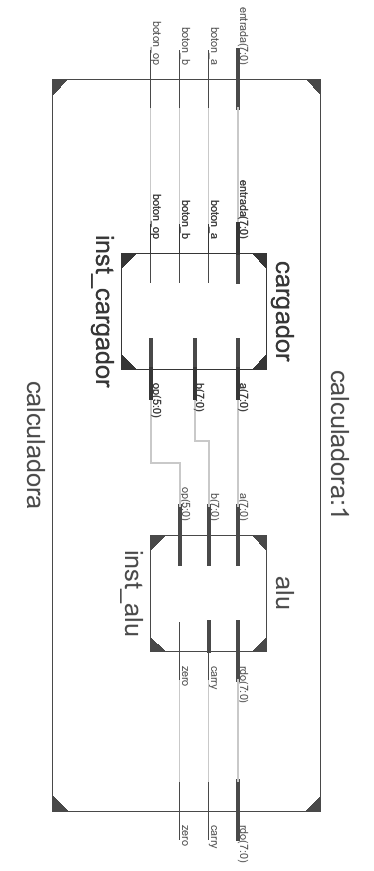
\includegraphics[height=0.5\textheight]{todo}}
\label{fig:todo}
\end{figure}

\section{Validación}
A continuación se muestran los resultados de los testbench
realizados sobre todas las operaciones implementadas, el código es el siguiente:
\begin{lstlisting}
module ALU_tb;

	// Inputs
	reg [7:0] entrada;
	reg boton_a;
	reg boton_b;
	reg boton_op;

	// Outputs
	wire [7:0] rdo;
	wire carry;
	wire zero;

	// Instantiate the Unit Under Test (UUT)
	calculadora uut (
		.entrada(entrada), 
		.boton_a(boton_a), 
		.boton_b(boton_b), 
		.boton_op(boton_op), 
		.rdo(rdo), 
		.carry(carry), 
		.zero(zero)
	);

	initial begin
		// Initialize Inputs
		entrada = 7;
		boton_a = 1;
		#20
		boton_a = 0;
		entrada = 5;
		boton_b = 1;
		#20
		boton_b = 0;
		entrada = 8'b00100000; //ADD
		boton_op = 1;

		// Wait 100 ns for global reset to finish
		#20;
        
		// Add stimulus here

	end
      
endmodule
\end{lstlisting}

Para las pruebas se fueron cambiando los valores de “entrada”, 
para cargar los registros con los valores que prueben mejor cada una de las operaciones.

\verb+ADD (binario 100000)+\\

\begin{center}
	\begin{tabular}{|c|c|}
		\hline 
		Variable & Valor\tabularnewline
		\hline 
		\hline 
		a & 250\tabularnewline
		\hline 
		b & 20\tabularnewline
		\hline 
		op & 100000\tabularnewline
		\hline 
		resultado & 14 + (carry)\tabularnewline
		\hline 
	\end{tabular}
\end{center}

Teniendo en cuenta el carry (256 por ser bit 9) mas 14 se tiene 270.

\begin{figure}[H] % Example image
\center{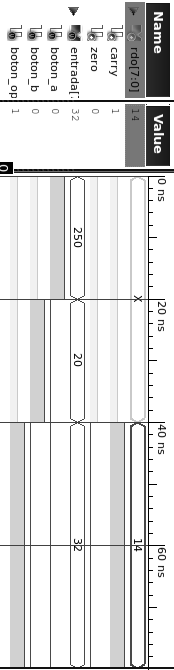
\includegraphics[height=0.4\textheight]{test1}}
\label{fig:test1}
\end{figure}

\verb+SUB (binario 100010)+\\

\begin{center}
	\begin{tabular}{|c|c|}
		\hline 
		Variable & Valor\tabularnewline
		\hline 
		\hline 
		a & 250\tabularnewline
		\hline 
		b & 20\tabularnewline
		\hline 
		op & 100010\tabularnewline
		\hline 
		resultado & 230\tabularnewline
		\hline 
	\end{tabular}
\end{center}


\begin{figure}[H] % Example image
\center{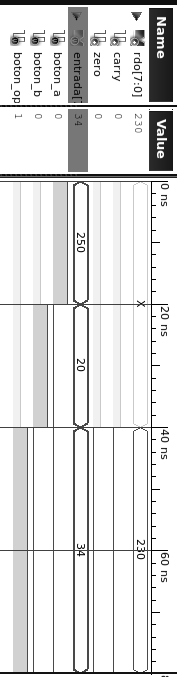
\includegraphics[height=0.4\textheight]{test2}}
\label{fig:test2}
\end{figure}

\verb+AND (binario 100100)+\\

\begin{center}
	\begin{tabular}{|c|c|}
		\hline 
		Variable & Valor\tabularnewline
		\hline 
		\hline 
		a & 10101010\tabularnewline
		\hline 
		b & 11110000\tabularnewline
		\hline 
		op & 100100\tabularnewline
		\hline 
		resultado & 10100000\tabularnewline
		\hline 
	\end{tabular}
\end{center}

\begin{figure}[H] % Example image
\center{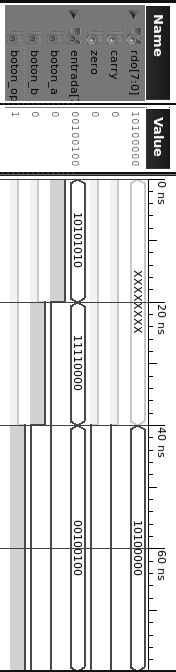
\includegraphics[height=0.4\textheight]{test3}}
\label{fig:test3}
\end{figure}

\verb+OR (binario 100101)+\\

\begin{center}
	\begin{tabular}{|c|c|}
		\hline 
		Variable & Valor\tabularnewline
		\hline 
		\hline 
		a & 10101010\tabularnewline
		\hline 
		b & 11110000\tabularnewline
		\hline 
		op & 100101\tabularnewline
		\hline 
		resultado & 11111010\tabularnewline
		\hline 
	\end{tabular}
\end{center}

\begin{figure}[H] % Example image
\center{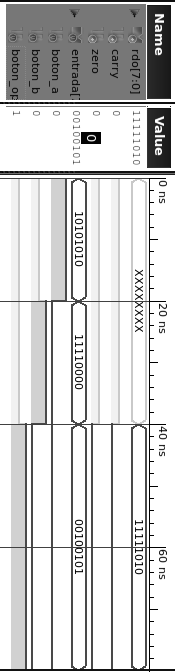
\includegraphics[height=0.4\textheight]{test4}}
\label{fig:test4}
\end{figure}

\verb+XOR (binario 100110)+\\

\begin{center}
	\begin{tabular}{|c|c|}
		\hline 
		Variable & Valor\tabularnewline
		\hline 
		\hline 
		a & 10101010\tabularnewline
		\hline 
		b & 11110000\tabularnewline
		\hline 
		op & 100110\tabularnewline
		\hline 
		resultado & 01011010\tabularnewline
		\hline 
	\end{tabular}
\end{center}

\begin{figure}[H] % Example image
\center{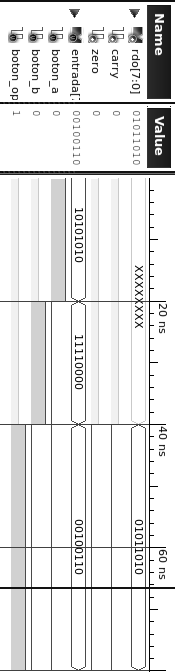
\includegraphics[height=0.4\textheight]{test5}}
\label{fig:test5}
\end{figure}

\verb+NOR (binario 100111)+\\

\begin{center}
	\begin{tabular}{|c|c|}
		\hline 
		Variable & Valor\tabularnewline
		\hline 
		\hline 
		a & 10101010\tabularnewline
		\hline 
		b & 11110000\tabularnewline
		\hline 
		op & 100111\tabularnewline
		\hline 
		resultado & 01011010\tabularnewline
		\hline 
	\end{tabular}
\end{center}

\begin{figure}[H] % Example image
\center{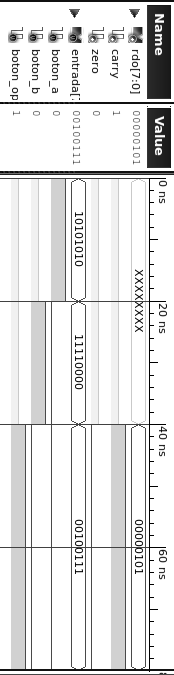
\includegraphics[height=0.4\textheight]{test6}}
\label{fig:test6}
\end{figure}

\verb+SRA (binario 000011)+\\

\begin{center}
	\begin{tabular}{|c|c|}
		\hline 
		Variable & Valor\tabularnewline
		\hline 
		\hline 
		a & 10101010\tabularnewline
		\hline 
		b & 11110000\tabularnewline
		\hline 
		op & 000011\tabularnewline
		\hline 
		resultado & 11000011\tabularnewline
		\hline 
	\end{tabular}
\end{center}

\begin{figure}[H] % Example image
\center{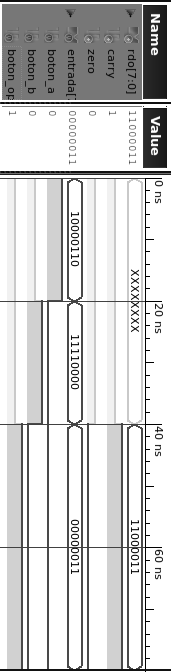
\includegraphics[height=0.4\textheight]{test7}}
\label{fig:test7}
\end{figure}

Tener en cuenta que el valor de b no se utiliza en esta operación, el shift siempre es de un bit. Además observar que se mantuvo el 1 en el bit mas significativo, en la próxima prueba se pone 0 como bit mas significativo de “a” para hacer énfasis en la diferencia.

\begin{center}
	\begin{tabular}{|c|c|}
		\hline 
		Variable & Valor\tabularnewline
		\hline 
		\hline 
		a & 00000110\tabularnewline
		\hline 
		b & 11110000\tabularnewline
		\hline 
		op & 000011\tabularnewline
		\hline 
		resultado & 00000011\tabularnewline
		\hline 
	\end{tabular}
\end{center}

\begin{figure}[H] % Example image
\center{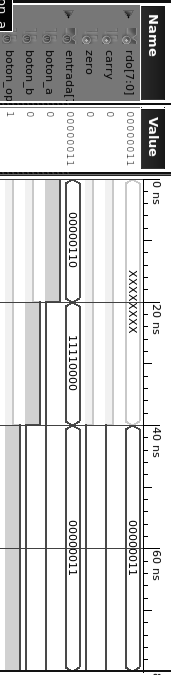
\includegraphics[height=0.4\textheight]{test8}}
\label{fig:test8}
\end{figure}

\verb+SRL (binario 000010)+\\

\begin{center}
	\begin{tabular}{|c|c|}
		\hline 
		Variable & Valor\tabularnewline
		\hline 
		\hline 
		a & 10000110\tabularnewline
		\hline 
		b & 11110000\tabularnewline
		\hline 
		op & 000010\tabularnewline
		\hline 
		resultado & 10100000\tabularnewline
		\hline 
	\end{tabular}
\end{center}

\begin{figure}[H] % Example image
\center{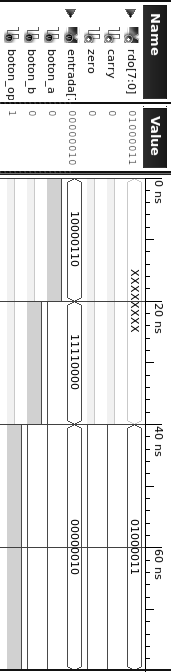
\includegraphics[height=0.4\textheight]{test9}}
\label{fig:test9}
\end{figure}

Al igual que SRA el valor de “b” no se tiene en cuenta en la operación. 
Observar que en este caso se relleno con cero lógico en vez de mantener el bit mas significativo.

\end{document}

%%% Local Variables: 
%%% mode: latex
%%% TeX-master: t
%%% End: 